% Options for packages loaded elsewhere
\PassOptionsToPackage{unicode}{hyperref}
\PassOptionsToPackage{hyphens}{url}
%
\documentclass[
  10pt,
  french,
  a5paper,
  openany]{book}
\usepackage{lmodern}
\usepackage{amssymb,amsmath}
\usepackage{ifxetex,ifluatex}
\ifnum 0\ifxetex 1\fi\ifluatex 1\fi=0 % if pdftex
  \usepackage[T1]{fontenc}
  \usepackage[utf8]{inputenc}
  \usepackage{textcomp} % provide euro and other symbols
\else % if luatex or xetex
  \usepackage{unicode-math}
  \defaultfontfeatures{Scale=MatchLowercase}
  \defaultfontfeatures[\rmfamily]{Ligatures=TeX,Scale=1}
\fi
% Use upquote if available, for straight quotes in verbatim environments
\IfFileExists{upquote.sty}{\usepackage{upquote}}{}
\IfFileExists{microtype.sty}{% use microtype if available
  \usepackage[]{microtype}
  \UseMicrotypeSet[protrusion]{basicmath} % disable protrusion for tt fonts
}{}
\makeatletter
\@ifundefined{KOMAClassName}{% if non-KOMA class
  \IfFileExists{parskip.sty}{%
    \usepackage{parskip}
  }{% else
    \setlength{\parindent}{0pt}
    \setlength{\parskip}{6pt plus 2pt minus 1pt}}
}{% if KOMA class
  \KOMAoptions{parskip=half}}
\makeatother
\usepackage{xcolor}
\IfFileExists{xurl.sty}{\usepackage{xurl}}{} % add URL line breaks if available
\IfFileExists{bookmark.sty}{\usepackage{bookmark}}{\usepackage{hyperref}}
\hypersetup{
  pdftitle={Travaux de maturité 2023},
  pdflang={fr},
  hidelinks,
  pdfcreator={LaTeX via pandoc}}
\urlstyle{same} % disable monospaced font for URLs
\usepackage[margin=20mm]{geometry}
\usepackage{longtable,booktabs}
% Correct order of tables after \paragraph or \subparagraph
\usepackage{etoolbox}
\makeatletter
\patchcmd\longtable{\par}{\if@noskipsec\mbox{}\fi\par}{}{}
\makeatother
% Allow footnotes in longtable head/foot
\IfFileExists{footnotehyper.sty}{\usepackage{footnotehyper}}{\usepackage{footnote}}
\makesavenoteenv{longtable}
\usepackage{graphicx,grffile}
\makeatletter
\def\maxwidth{\ifdim\Gin@nat@width>\linewidth\linewidth\else\Gin@nat@width\fi}
\def\maxheight{\ifdim\Gin@nat@height>\textheight\textheight\else\Gin@nat@height\fi}
\makeatother
% Scale images if necessary, so that they will not overflow the page
% margins by default, and it is still possible to overwrite the defaults
% using explicit options in \includegraphics[width, height, ...]{}
\setkeys{Gin}{width=\maxwidth,height=\maxheight,keepaspectratio}
% Set default figure placement to htbp
\makeatletter
\def\fps@figure{htbp}
\makeatother
\setlength{\emergencystretch}{3em} % prevent overfull lines
\providecommand{\tightlist}{%
  \setlength{\itemsep}{0pt}\setlength{\parskip}{0pt}}
\setcounter{secnumdepth}{5}
\usepackage[T1]{fontenc}
\usepackage[]{plex-otf}
\renewcommand*\familydefault{\sfdefault}

\widowpenalty10000
\clubpenalty10000

\renewcommand{\arraystretch}{1.5}

\setcounter{tocdepth}{1}

\usepackage{booktabs}
\usepackage{tabto}

\usepackage{fancyhdr}
\setlength{\headheight}{15pt}

\pagestyle{fancy}
\lhead{}
\chead{}
\rhead{\footnotesize Travaux de maturité 2023}
\lfoot{}
\cfoot{\footnotesize\thepage}
\rfoot{}
\renewcommand{\headrulewidth}{0.2pt}
\renewcommand{\footrulewidth}{0.2pt}

\fancypagestyle{plain}{
  \pagestyle{fancy}
  \lhead{}
  \chead{}
  \rhead{}
  \lfoot{}
  \cfoot{\footnotesize\thepage}
  \rfoot{}
  \renewcommand{\headrulewidth}{0pt}
  \renewcommand{\footrulewidth}{0.2pt}
}

\usepackage{titlesec}
\titlespacing{\chapter}{0em}{0em}{1em}
\titleformat{\chapter}[display]{\normalfont\bfseries\centering}{}{0pt}{\Large}
\titleformat{\section}[display]{\normalfont\bfseries}{}{0pt}{\large}
\titleformat{\subsection}[display]{\normalfont\bfseries}{}{0pt}{\normalsize}

\newenvironment{signature}{\begin{flushright}}{\end{flushright}}
\ifxetex
  % Load polyglossia as late as possible: uses bidi with RTL langages (e.g. Hebrew, Arabic)
  \usepackage{polyglossia}
  \setmainlanguage[]{french}
\else
  \usepackage[shorthands=off,main=french]{babel}
\fi

\title{Travaux de maturité 2023}
\author{}
\date{\vspace{-2.5em}30.10.2022}

\begin{document}
\maketitle

{
\setcounter{tocdepth}{0}
\tableofcontents
}
\hypertarget{le-mot-du-doyen}{%
\chapter*{Le mot du doyen}\label{le-mot-du-doyen}}
\addcontentsline{toc}{chapter}{Le mot du doyen}

\begin{figure}


\includegraphics[height=5em]{images/logoGNLC} \hfill{}

\end{figure}

\vspace{\stretch{1}}

\begin{signature}
\emph{À toutes et tous les élèves}\\
\emph{des classes de 2\textsuperscript{e} année}\\
\emph{de l'École de maturité}

\end{signature}

\vspace{\stretch{1}}

Chères élèves, chers élèves,

Vous recevez cette brochure qui concerne le travail de maturité pour la volée 2022-2023 et qui contient, en particulier, les thèmes des projets qui vous sont proposés.

Je vous donne rendez-vous le

\begin{center}
\textbf{Mardi 22 novembre à 11h05 ;\\
Espace Assemblée (en prolongement de la cafétéria)}

\end{center}

afin d'y recevoir une information générale sur l'organisation du travail de maturité.

Vous aurez ensuite la possibilité de suivre la présentation de trois projets que vous aurez retenus parmi les pages qui suivent. Les présentations se dérouleront comme suit :

\begin{itemize}
\tightlist
\item
  la première de 11h55 à 12h20,
\item
  la seconde de 12h25 à 12h50 et
\item
  la troisième de 12h55 à 13h30.
\end{itemize}

Les cours seront donc interrompus ce jour de 10h50 à 13h30 pour les classes de 2M. Ils reprendront à 13h35 selon l'horaire habituel.

\clearpage

Après ces présentations, vous aurez à choisir trois thèmes. Vous devrez vous inscrire via le site du Gymnase de Nyon (\url{www.gymnasedenyon.ch}) en cliquant dans le menu

\begin{center}
``Intranet \textgreater{} Elèves \textgreater{} Horaires et Inscriptions'' puis ``Inscriptions''

\end{center}

et en respectant le délai fixé au \textbf{mercredi 30 novembre à 16h00}. Vous devrez formuler 3 souhaits, dans l'ordre de préférence. Les inscriptions définitives vous seront confirmées ultérieurement.

Avec mes meilleures salutations,

\begin{signature}
Le doyen\\
M. Rizzello

\end{signature}

\vspace{\stretch{1}}

Distribution à :

\begin{itemize}
\tightlist
\item
  toutes les classes de 2M
\item
  Conseil de direction
\item
  Mmes et MM. les maître·sse·s de classe de 2M
\item
  Mmes et MM. les responsables de projets, avec prière d'assister à cette séance d'information et de présenter les propositions de projets dans les salles qui seront attribuées
\end{itemize}

\hypertarget{attribution-des-salles}{%
\chapter*{Attribution des salles}\label{attribution-des-salles}}
\addcontentsline{toc}{chapter}{Attribution des salles}

\begin{longtable}[]{@{}lc@{}}
\toprule
Thème & Salle n°\tabularnewline
\midrule
\endhead
Philosophie de l'art : La beauté et la vérité & \textasciitilde{}\tabularnewline
Le récit de voyage & \textasciitilde{}\tabularnewline
Le jeu vidéo : fiction ou réalité ? & \textasciitilde{}\tabularnewline
Des analyses chimiques avec mon téléphone portable & \textasciitilde{}\tabularnewline
Chimie et photographie & \textasciitilde{}\tabularnewline
L'eau chaude gèle-t-elle plus vite que l'eau froide ? & \textasciitilde{}\tabularnewline
\bottomrule
\end{longtable}

\hypertarget{rappel-des-dispositions-ruxe8glementaires}{%
\chapter*{Rappel des dispositions règlementaires}\label{rappel-des-dispositions-ruxe8glementaires}}
\addcontentsline{toc}{chapter}{Rappel des dispositions règlementaires}

\hypertarget{ruxe8glement-du-16-janvier-1995-sur-la-reconnaissance-des-certificats-de-maturituxe9-gymnasiale-rrm}{%
\subsection*{Règlement du 16 janvier 1995 sur la reconnaissance des certificats de maturité gymnasiale (RRM)}\label{ruxe8glement-du-16-janvier-1995-sur-la-reconnaissance-des-certificats-de-maturituxe9-gymnasiale-rrm}}
\addcontentsline{toc}{subsection}{Règlement du 16 janvier 1995 sur la reconnaissance des certificats de maturité gymnasiale (RRM)}

\emph{{[}édicté par la Conférence suisse des Directeurs cantonaux de l'instruction publique (CDIP) ; état au 1er août 2007{]}}

\vspace{\stretch{1}}

\emph{Art. 9 Disciplines de maturité}

\begin{enumerate}
\def\labelenumi{\arabic{enumi}.}
\tightlist
\item
  Les disciplines fondamentales, l'option spécifique, l'option complémentaire et le travail de maturité constituent l'ensemble des disciplines de la maturité.
\end{enumerate}

(\ldots)

\vspace{\stretch{1}}

\emph{Art. 10 Travail de maturité}

Chaque élève doit effectuer, seul ou en équipe, un travail autonome d'une certaine importance. Ce travail fera l'objet d'un texte ou d'un commentaire rédigé et d'une présentation orale.

\vspace{\stretch{1}}

\emph{Art.15 Notes de maturité et évaluation du travail de maturité}

(\ldots)

\begin{enumerate}
\def\labelenumi{\arabic{enumi}.}
\setcounter{enumi}{1}
\tightlist
\item
  Le travail de maturité est évalué sur la base des prestations écrites et orales.
\end{enumerate}

\vspace{\stretch{1}}

\clearpage

\hypertarget{ruxe8glement-des-gymnases-du-6-juillet-2016-rgy}{%
\subsection*{Règlement des gymnases du 6 juillet 2016 (RGY)}\label{ruxe8glement-des-gymnases-du-6-juillet-2016-rgy}}
\addcontentsline{toc}{subsection}{Règlement des gymnases du 6 juillet 2016 (RGY)}

\emph{{[}édicté par le Conseil d'État du Canton de Vaud{]}}

\emph{Art.82 Travail de maturité}

\begin{enumerate}
\def\labelenumi{\arabic{enumi}.}
\tightlist
\item
  Les élèves effectuent un travail de maturité, seuls ou en équipe, entre la 2ème etla 3ème années, selon le calendrier fixé par le directeur et les modalités fixées par le département.
\item
  Le travail de maturité est évalué par un jury interne qui peut, le cas échéant, s'adjoindre un expert externe, sur la base de la mise en œuvre du projet, du document écrit déposé et de la présentation orale.
\item
  Le travail de maturité donne lieu à une note annuelle en 3ème année.
\item
  Le titre du travail de maturité est mentionné sur le certificat de maturité gymnasiale.
\item
  L'élève qui répète la 3ème année choisit, pour le début de l'année scolaire, soit de conserver sa note, soit d'effectuer un nouveau travail de maturité. Dans ce dernier cas, la note attribuée au premier travail n'est pas conservée.
\end{enumerate}

(\ldots)

\hypertarget{objectifs-et-uxe9valuation}{%
\chapter*{Objectifs et évaluation}\label{objectifs-et-uxe9valuation}}
\addcontentsline{toc}{chapter}{Objectifs et évaluation}

\hypertarget{principes-fondamentaux}{%
\section*{Principes fondamentaux}\label{principes-fondamentaux}}
\addcontentsline{toc}{section}{Principes fondamentaux}

Le travail de maturité est l'occasion pour l'élève, à l'issue d'un processus de longue durée, de parvenir à une assise, une ``maturité'' intellectuelle suffisamment solide pour pouvoir produire un discours ou une œuvre qu'il peut assumer en tant qu'auteur et soumettre au regard d'autrui. En d'autres termes, il s'agit pour lui de se constituer comme sujet d'une énonciation.

\hypertarget{objectifs-fondamentaux}{%
\section*{Objectifs fondamentaux}\label{objectifs-fondamentaux}}
\addcontentsline{toc}{section}{Objectifs fondamentaux}

Fondamentalement, il doit, pour parvenir à cela, être capable de :

\begin{itemize}
\tightlist
\item
  mener une recherche documentaire de qualité ;
\item
  structurer sa pensée, afin de progresser vers un but, qui consiste à résoudre un problème ;
\item
  formuler sa pensée pour la rendre intelligible à autrui ;
\item
  évaluer sa propre démarche et distinguer clairement sa position personnelle d'autres points de vue, en justifiant ses choix.
\end{itemize}

\hypertarget{uxe9valuation}{%
\section*{Évaluation}\label{uxe9valuation}}
\addcontentsline{toc}{section}{Évaluation}

\hypertarget{relation-puxe9dagogique}{%
\subsection*{Relation pédagogique}\label{relation-puxe9dagogique}}
\addcontentsline{toc}{subsection}{Relation pédagogique}

Le travail de maturité s'élabore sous la conduite d'un maître répondant. Il s'agit d'un processus de longue durée, qui doit être considéré comme une situation d'enseignement, ce qui implique un suivi et des échanges réguliers entre le répondant et l'élève.

En entreprenant son travail de maturité, l'élève s'engage dans une relation de collaboration avec son répondant : cela suppose que le contact soit cultivé de part et d'autre.

\hypertarget{uxe9valuation-1}{%
\subsection*{Évaluation}\label{uxe9valuation-1}}
\addcontentsline{toc}{subsection}{Évaluation}

L'évaluation du travail de maturité (travail d'analyse ou de création) porte sur les six domaines de compétence suivants :

\begin{itemize}
\tightlist
\item
  Recherche et méthodes de travail
\item
  Contenu et sens
\item
  Structure de l'opuscule
\item
  Sens critique, lucidité sur son travail
\item
  Expression
\item
  Présentation
\end{itemize}

\hypertarget{calendrier-pour-la-voluxe9e-2023}{%
\chapter*{Calendrier pour la volée 2023}\label{calendrier-pour-la-voluxe9e-2023}}
\addcontentsline{toc}{chapter}{Calendrier pour la volée 2023}

\vspace{\stretch{1}}

\textbf{1. Phase préparatoire \hfill septembre - décembre 2022}

\begin{longtable}[]{@{}ll@{}}
\toprule
\endhead
Propositions de projets &\tabularnewline
Constitution des équipes de projets &\tabularnewline
Information générale aux élèves de 2M &\tabularnewline
Présentation des projets par les équipes de maîtres &\tabularnewline
Inscription &\tabularnewline
\bottomrule
\end{longtable}

\vspace{\stretch{1}}

\textbf{2. Élaboration des sujets \hfill février - mars 2023}

\begin{longtable}[]{@{}ll@{}}
\toprule
\endhead
\begin{minipage}[t]{0.65\columnwidth}\raggedright
Élaboration et choix des sujets par les élèves\strut
\end{minipage} & \begin{minipage}[t]{0.29\columnwidth}\raggedright
semaine spéciale : 3 et 6, 7, 8 février 2023\strut
\end{minipage}\tabularnewline
\begin{minipage}[t]{0.65\columnwidth}\raggedright
Signature de l'engagement par les élèves et confirmation des répondants (à remettre au secrétariat)\strut
\end{minipage} & \begin{minipage}[t]{0.29\columnwidth}\raggedright
dernier délai : 6 mars 2023\strut
\end{minipage}\tabularnewline
\bottomrule
\end{longtable}

\vspace{\stretch{1}}

\clearpage

\vspace{\stretch{1}}

\textbf{3. Réalisation des projets \hfill mars - novembre 2023}

\begin{longtable}[]{@{}ll@{}}
\toprule
\endhead
\begin{minipage}[t]{0.67\columnwidth}\raggedright
1ère évaluation intermédiaire, fiche remise aux élèves avant les vacances d'été\strut
\end{minipage} & \begin{minipage}[t]{0.27\columnwidth}\raggedright
juin 2023\strut
\end{minipage}\tabularnewline
\begin{minipage}[t]{0.67\columnwidth}\raggedright
2ème évaluation intermédiaire, fiche remise aux élèves avant le 1er octobre\strut
\end{minipage} & \begin{minipage}[t]{0.27\columnwidth}\raggedright
2ème quinzaine de septembre 2023\strut
\end{minipage}\tabularnewline
\begin{minipage}[t]{0.67\columnwidth}\raggedright
Remise des travaux dans leur forme définitive\strut
\end{minipage} & \begin{minipage}[t]{0.27\columnwidth}\raggedright
lundi 13 novembre 2023\strut
\end{minipage}\tabularnewline
\bottomrule
\end{longtable}

\vspace{\stretch{1}}

\textbf{4. Évaluation finale \hfill novembre - décembre 2023}

\begin{longtable}[]{@{}ll@{}}
\toprule
\endhead
\begin{minipage}[t]{0.56\columnwidth}\raggedright
Lecture des travaux de maturité par le jury\strut
\end{minipage} & \begin{minipage}[t]{0.38\columnwidth}\raggedright
\strut
\end{minipage}\tabularnewline
\begin{minipage}[t]{0.56\columnwidth}\raggedright
Défense des travaux de maturité par les élèves\strut
\end{minipage} & \begin{minipage}[t]{0.38\columnwidth}\raggedright
1ère quinzaine de décembre 2023\strut
\end{minipage}\tabularnewline
\bottomrule
\end{longtable}

\vspace{\stretch{1}}

\fancypagestyle{themes}{
    \fancyhead[RO]{\footnotesize\leftmark}
}
\renewcommand{\chaptermark}[1]{\markboth{\footnotesize\space#1}{}}
\pagestyle{themes}

\hypertarget{philosophie-de-lart-la-beautuxe9-et-la-vuxe9rituxe9}{%
\chapter{Philosophie de l'art : La beauté et la vérité}\label{philosophie-de-lart-la-beautuxe9-et-la-vuxe9rituxe9}}

Que la beauté soit une affaire de goût, qu'elle soit subjective, qu'elle soit relative et propre à chacun, c'est ce qui semble aller de soi. Mais que dire du chef-d'œuvre qui prétend à l'universalité~? Que dire du jugement esthétique qui s'offusque lorsqu'on le contrarie~? Une fleur est belle, un paysage est beau, un visage est beau~: n'est-ce pas à dire que la beauté se situe dans les choses~? Qu'elle est objective~? Mais alors, comment se dévoile-t-elle~? Est-ce par une modification du regard chez l'observateur, par un travail de l'artiste sur la chose qu'il façonne, ou par l'éclat à peine aperçu d'un objet qui suggère qu'il dissimule un secret~? Pouvons-nous nous contenter de regarder une œuvre d'art ou devons-nous la contempler~? Et l'artiste, dès lors, est-il un créateur ou un voyant~? Il n'est pas rare d'ailleurs que nous ressentions un sentiment d'authenticité face à une œuvre d'art --~comme si là, en face de nous, c'était la vérité qui s'exprimait. Ce sentiment équivaut-il à une émotion~? Une réaction à une réalité qui donne des frissons~? Mais si c'est la vérité qui se manifeste dans une œuvre d'art~-- est-ce à dire que la science ne possède pas le monopole du savoir~? Que la science et l'art seraient des disciplines opposées, voire incompatibles~? Rien n'est moins sûr. Mais nous entendons que l'art a pour fonction d'imiter la nature, alors que la science l'explique et la décrit. Ne serait-ce pas que l'art a pour fonction d'embellir la nature~? Mais que dire alors des œuvres sublimes qui accentuent la laideur physique et la dégradation morale de ses sujets~? Que dire des caricatures, par exemple, desquelles se dégagent indiscutablement une modalité du beau et du vrai~? Accentuer les traits, déformer les corps, exagérer les expressions~: n'est-ce pas mentir~? Que dire des dissonances musicales qui semblent rompre un ordre harmonique qui est si doux à nos oreilles~? Représenter iconographiquement des êtres célestes et divins, n'est-ce pas profaner des entités qui dépassent la condition de l'homme~? Très rapidement s'est posée la question de savoir comment exprimer une idée artistique.

Nous pourrions en outre nous demander si l'expression artistique est une activité proprement humaine. Ne voyons-nous pas des araignées construire des édifices symétriques, dont la régularité surpassent parfois nos efforts architecturaux~? N'observons-nous pas dans la nature de nombreux actes de séduction animalière qui laissent entendre que les animaux possèdent aussi une sensibilité esthétique ? Peut-être que l'harmonie de la nature nous a conféré des normes artistiques dont il est difficile de nous défaire.

Tel serait un échantillon des questions qui peuvent être soulevées dans ce Travail de Maturité. Avec l'aide de textes appartenant à la tradition philosophique, mais aussi à la littérature, à la poésie, et aux artistes eux-mêmes --~qui ont souvent écrit sur leur pratique~--, nous nous interrogerons sur l'attrait qu'exerce sur nous le pouvoir des créations artistiques. Qu'il s'agisse du plaisir indescriptible qu'éveille la jouissance artistique, du moment de suspens que provoque en nous l'expérience esthétique elle-même, du basculement par lequel nous nous perdons dans un tableau, dans une sculpture, dans un morceau de musique, ou dans un film, du sérieux ou du jeu avec lesquels nous nous approchons d'une œuvre d'art, du milieu dans lequel l'œuvre d'art doit ou peut être appréhendée (théâtre, musée, chez soi, nature), de la modification que lui fait subir les impératifs de consommation, nous nous attacherons à montrer que la création artistique possède une place fondamentale dans notre rapport au monde.

Ce Travail de Maturité est ouvert à tous et n'exige aucun prérequis. Il demande simplement un intérêt pour la question artistique, une envie de penser, et une dose de curiosité.

\begin{signature}
\emph{J. Filthuth et E. Puric}

\end{signature}

\hypertarget{le-ruxe9cit-de-voyage}{%
\chapter{Le récit de voyage}\label{le-ruxe9cit-de-voyage}}

\begin{figure}

{\centering 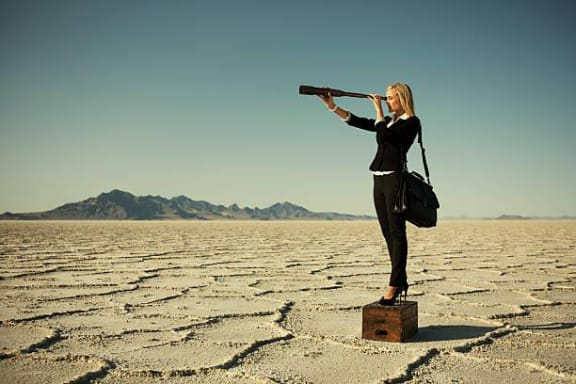
\includegraphics[height=12em]{images/le-recit-de-voyage} 

}

\end{figure}

De tous temps, nous, humains, avons ressenti l'appel du large et sommes partis à l'aventure vers des contrées inconnues pour en rapporter des histoires fantastiques. Le voyage permet de sortir de nos habitudes, de retrouver l'essentiel et parfois de nous donner l'illusion de la liberté.

Dans ce TM il s'agira de choisir votre propre destination pour ensuite en faire un récit de voyage. Nous aborderons le récit de voyage à travers des auteurs comme Sylvain Tesson, Ella Maillart ou d'autres écrivains. Puis ça sera à vous, par groupe de deux, d'organiser puis d'entamer votre voyage qui constituera la base de votre récit. Nul besoin d'aller à l'autre bout de la planète : il s'agit de sortir de son quotidien et de sa zone de confort et de partir à la découverte de lieux nouveaux qui nourrissent notre imaginaire. Vous en ferez ensuite votre propre récit de voyage, un texte écrit et agrémenté par exemple de photos, de vidéos ou de dessins pour à votre tour faire voyager vos lecteurs.

N.B. Ce TM peut se faire en français ou en anglais et doit être rédigé à deux.

\hypertarget{travel-literature}{%
\section*{Travel literature}\label{travel-literature}}
\addcontentsline{toc}{section}{Travel literature}

For ages, we have felt the call from the sea and have adventured towards unknown places coming back to narrate our incredible experiences. Traveling allows us to escape from our habits, find what's essential and sometimes gives us the illusion of being free.

In this TM you will discover what travel literature is, through texts by Sylvain Tesson, Ella Maillart or other writers. Then it will be your turn, in groups of two, to organise and start off your own travel adventure which will be the starting point of your text. No need to go far away: it's about leaving our daily routine and comfort zone to discover new places that fuel our imagination. You will then produce a written text on your travel adding for example photos, videos and drawings to make your readers travel as well.

N.B. This TM can be written in French or English and needs to be done in groups of two.

\begin{signature}
\emph{J. Menamkat}

\end{signature}

\hypertarget{le-jeu-viduxe9o-fiction-ou-ruxe9alituxe9}{%
\chapter{Le jeu vidéo : fiction ou réalité~?}\label{le-jeu-viduxe9o-fiction-ou-ruxe9alituxe9}}

\begin{figure}

{\centering 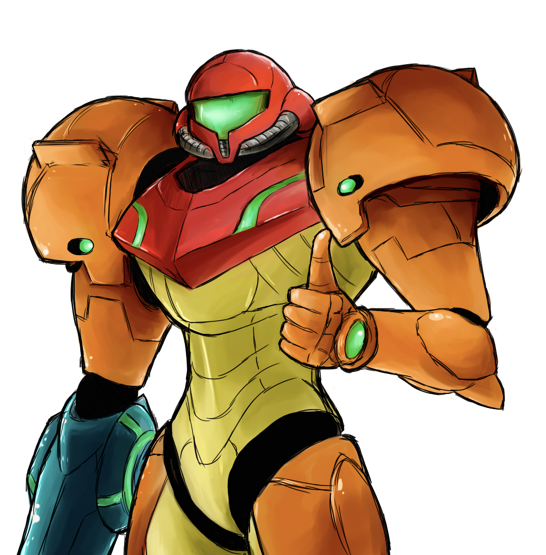
\includegraphics[height=12em]{images/le-jeu-video-fiction-ou-realite} 

}

\end{figure}

\vspace{\stretch{1}}

Depuis une dizaine d'années, la pratique du jeu vidéo s'est répandue à une large partie de la population. Bien que de nombreuses personnes aient accusé ce divertissement d'être à l'origine de violences ou de provoquer l'isolement des gameurs-euses, nous parlons actuellement du 10\textsuperscript{e} art pour nommer les jeux vidéo.

La stratégie de cette industrie ne repose pas uniquement sur le degré de divertissement qu'ils procurent, mais également sur leur impact visuel comme intellectuel. Ainsi a-t-on réalisé d'impressionnants progrès dans le développement réaliste des graphiques et dans la complexité de leur scénario.

Tout en laissant place à des produits originaux et conceptuels, les développeurs-ses tendent donc à mêler le réel à la fiction en ouvrant le champ à de nouvelles réflexions : comment représenter la société, le genre, la femme~? Comment simuler l'histoire, la gestion, les métiers~? Comment vous permettre à vous, gameurs-euses, de vous plonger dans un divertissement si immersif qu'il vous ouvre les portes d'une nouvelle dimension~?

\clearpage

La finalité de ce travail de maturité est d'étudier la limite entre la réalité et la fiction dans le jeu vidéo. Ce sujet, vaste, vous laisse donc la liberté de proposer diverses problématiques faisant appel à votre pratique, hautement recommandée, des jeux vidéo.

\begin{signature}
\emph{A. Morier et L. Moser}

\end{signature}

\begin{figure}

\hfill{}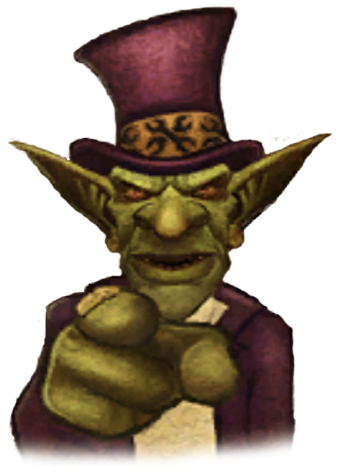
\includegraphics[height=7em]{images/le-jeu-video-fiction-ou-realite-2} 

\end{figure}

\hypertarget{des-analyses-chimiques-avec-mon-tuxe9luxe9phone-portable}{%
\chapter{Des analyses chimiques avec mon téléphone portable}\label{des-analyses-chimiques-avec-mon-tuxe9luxe9phone-portable}}

\begin{figure}

{\centering 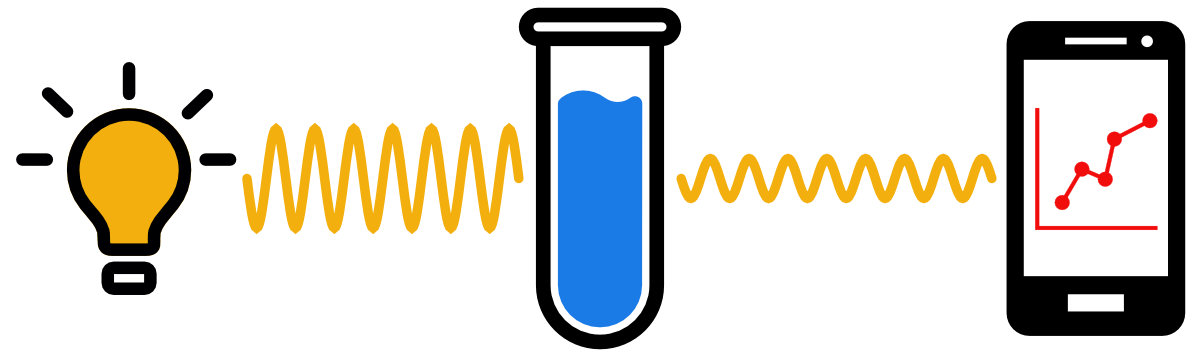
\includegraphics[height=12em]{images/analyses-chimiques-telephone-portable} 

}

\end{figure}

Les smartphones font partie intégrante de notre vie quotidienne, mais nous accordons peu d'attention à l'utilisation de leurs capteurs pour la collecte et l'analyse de données. En effet, ces appareils intègrent généralement un capteur d'image, un microphone, un accéléromètre, un gyroscope, un capteur de pression atmosphérique, une boussole numérique et bien d'autres instruments encore qui peuvent être extrêmement utiles dans un laboratoire de chimie.

Alors, pourquoi s'en priver et ne pas utiliser ces puissants appareils qui tiennent dans le creux de notre main pour résoudre des problèmes du laboratoire ?

La colorimétrie est une méthode d'analyse qui relie la variation de la couleur d'une solution à la concentration d'un soluté. Un colorimètre est un appareil coûteux et très utilisé en chimie et en biologie pour, par exemple, l'analyse du sang ou de l'eau, des nutriments du sol et des denrées alimentaires, la détermination des vitesses de réaction ou l'étude de la croissance de cultures bactériennes.

Ce thème de travail de maturité vous propose de concevoir et développer un dispositif d'analyse chimique permettant de transformer simplement n'importe quel téléphone portable en un colorimètre fiable.

\begin{signature}
\emph{M. Rizzello}

\end{signature}

\hypertarget{chimie-et-photographie}{%
\chapter{Chimie et photographie}\label{chimie-et-photographie}}

\begin{figure}

{\centering 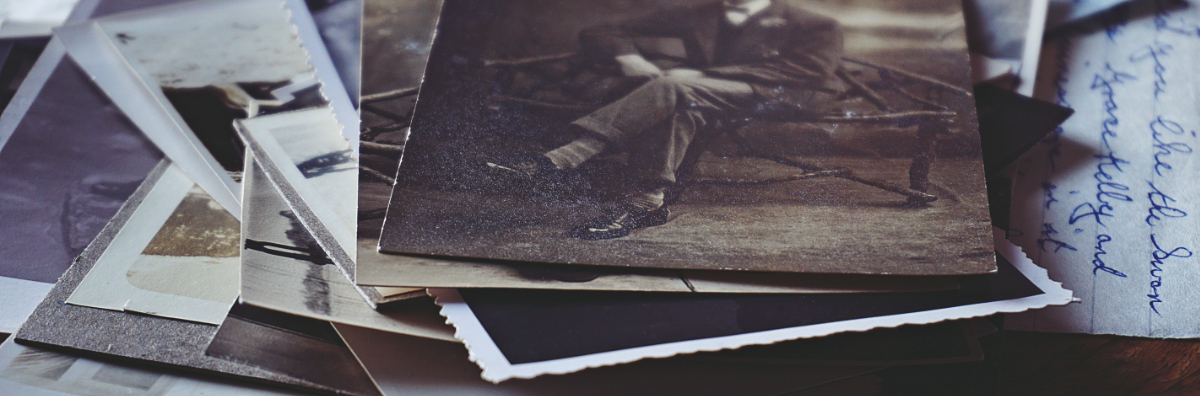
\includegraphics[height=10em]{images/chimie-et-photographie} 

}

\end{figure}

\vspace{\stretch{1}}

\hypertarget{un-sujet-pour-les-uxe9luxe8ves-photosensibles}{%
\subsection*{Un sujet pour les élèves photosensibles}\label{un-sujet-pour-les-uxe9luxe8ves-photosensibles}}
\addcontentsline{toc}{subsection}{Un sujet pour les élèves photosensibles}

Les nouvelles technologies permettent d'avoir en permanence sur soi un appareil photo. Lorsque nous prenons une photo, nous sommes aujourd'hui habitués à une récompense instantanée~: on regarde un écran numérique, on clique sur un bouton et l'on obtient une image parfaite. Mais il n'en a pas toujours été ainsi~\ldots{}

Ce thème de travail de maturité est une exploration de la chimie de la photographie par l'expérience pratique. Vous élargirez vos connaissances de la technique photographique et de la fabrication de tirages, tout en appliquant la chimie que vous apprenez en cours.

L'objectif du projet est de recréer un ou plusieurs procédés chimiques traditionnellement utilisés pour le développement avec des produits domestiques de substitution et être capable d'expliquer, grâce à leurs propriétés chimiques, pourquoi ces substitutions fonctionnent. Le produit fini sera un procédé que n'importe qui pourrait créer, sans accéder à des fournitures photographiques coûteuses.

\begin{signature}
\emph{M. Rizzello}

\end{signature}

\hypertarget{leau-chaude-guxe8le-t-elle-plus-vite-que-leau-froide}{%
\chapter{L'eau chaude gèle-t-elle plus vite que l'eau froide~?}\label{leau-chaude-guxe8le-t-elle-plus-vite-que-leau-froide}}

\begin{figure}

{\centering 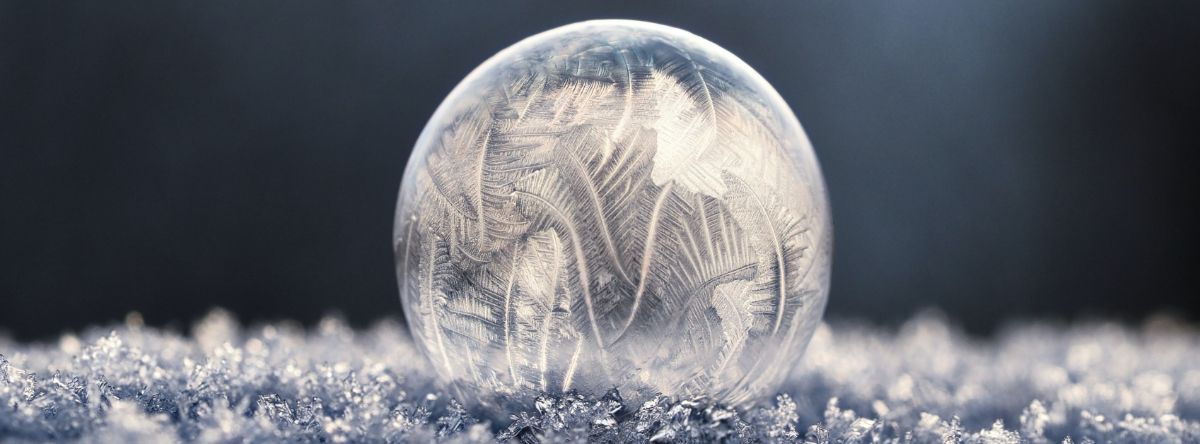
\includegraphics[height=12em]{images/eau-chaude} 

}

\end{figure}

On pourrait dire que c'est une des expériences les plus simples qui soient. Prenez deux récipients, un rempli d'eau chaude et l'autre rempli d'eau froide. Placez-les dans un congélateur et notez laquelle gèle en premier. Le bon sens suggère que l'eau froide gèlera en premier. Cependant, depuis l'Antiquité, on observe que, sous certaines conditions, l'eau chaude peut refroidir plus vite.

Ce phénomène a été porté à l'attention du public en 1963 par un étudiant tanzanien de 17 ans, Erasto Mpemba. Accidentellement, il a découvert que la glace qu'il avait fabriquée en congelant un mélange chaud avait gelé avant celle de ses camarades, réalisée avec des mélanges froids. Quand il raconta à son professeur ce qu'il avait observé, le professeur lui dit qu'il avait dû se tromper. Personne ne l'a cru.

Mpemba n'a pas baissé les bras et a présenté ses observations à un professeur d'université qui visitait son école. Le professeur a tenté l'expérience, il l'a confirmée et ils ont ensuite coécrit un article à ce sujet qui fut en 1969. Au fil des ans, de nombreuses personnes ont essayé de reproduire cette expérience, certaines ont réussi et d'autres ont échoué. Aujourd'hui encore, il existe une controverse sur les bases théoriques et sur les paramètres nécessaires pour reproduire cet effet.

Le but de ce travail de maturité sera de concevoir et tester un dispositif technique permettant d'observer le phénomène et de tenter de fournir une explication à cet effet, connu aujourd'hui sous le nom d'effet Mpemba.

\begin{signature}
\emph{M. Rizzello}

\end{signature}

\hypertarget{le-conte-uxe9crit-transposuxe9-au-cinuxe9ma}{%
\chapter{Le conte écrit transposé au cinéma}\label{le-conte-uxe9crit-transposuxe9-au-cinuxe9ma}}

\begin{figure}

{\centering 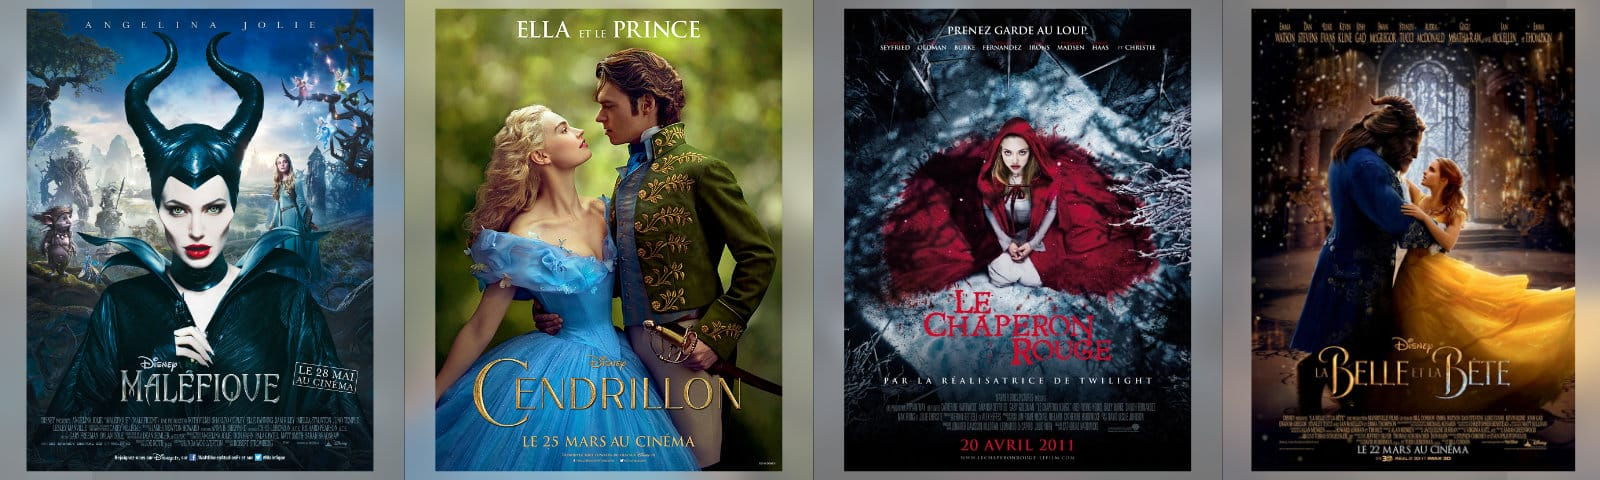
\includegraphics[height=10em]{images/le-conte-ecrit-transpose-au-cinema} 

}

\end{figure}

La réalisation d'un film implique nécessairement une adaptation. Parfois les modifications apportées (titre, durée d'une action, lieux, les dialogues, enchaînements, etc.) sont telles que le film devient une œuvre nouvelle.
Il y a également une modification du point de vue du spectateur, dont la liberté interprétative est restreinte face à une mise en scène choisie.

\hypertarget{contes-et-leur-adaptation-cinuxe9matographique}{%
\subsection*{Contes et leur adaptation cinématographique}\label{contes-et-leur-adaptation-cinuxe9matographique}}
\addcontentsline{toc}{subsection}{Contes et leur adaptation cinématographique}

\begin{longtable}[]{@{}ll@{}}
\toprule
\begin{minipage}[b]{0.51\columnwidth}\raggedright
Conte\strut
\end{minipage} & \begin{minipage}[b]{0.43\columnwidth}\raggedright
Adaptation\strut
\end{minipage}\tabularnewline
\midrule
\endhead
\begin{minipage}[t]{0.51\columnwidth}\raggedright
La belle au bois dormant,\linebreak Charles Perrault\strut
\end{minipage} & \begin{minipage}[t]{0.43\columnwidth}\raggedright
Maléfique\linebreak (2014, Robert Stromberg)\strut
\end{minipage}\tabularnewline
\begin{minipage}[t]{0.51\columnwidth}\raggedright
Cendrillon,\linebreak Charles Perrault\strut
\end{minipage} & \begin{minipage}[t]{0.43\columnwidth}\raggedright
Cendrillon\linebreak (2015, Kenneth Branagh)\strut
\end{minipage}\tabularnewline
\begin{minipage}[t]{0.51\columnwidth}\raggedright
Le Petit Chaperon rouge,\linebreak Charles Perrault\strut
\end{minipage} & \begin{minipage}[t]{0.43\columnwidth}\raggedright
Le Chaperon Rouge\linebreak (2011, Catherine Hardwicke)\strut
\end{minipage}\tabularnewline
\begin{minipage}[t]{0.51\columnwidth}\raggedright
La Belle et la Bête,\linebreak Jeanne-Marie Leprince de Beaumont\strut
\end{minipage} & \begin{minipage}[t]{0.43\columnwidth}\raggedright
La Belle et la Bête\linebreak (2017, Bill Condon)\strut
\end{minipage}\tabularnewline
\bottomrule
\end{longtable}

\clearpage

Le sujet proposé vous permet d'explorer les différences entre un conte écrit et son adaptation cinématographique, à partir d'une thématique, d'un motif ou d'un autre point de comparaison. Pour ce faire, vous choisirez quelques extraits de texte au sein d'un conte afin de les mettre en parallèle avec les séquences du film correspondantes.

\begin{signature}
\emph{S. Alves}

\end{signature}

\end{document}
